\documentclass{beamer}
%% \usetheme{Warsaw}
\usepackage{etex}
\usepackage{ulem}

\renewcommand<>{\sout}[1]{
  \only#2{\beameroriginal{\sout}{#1}}
  \invisible#2{#1}
}

\usepackage{color}
\usepackage{booktabs}
\usepackage{tikz}
\usepackage{pgfplots}
\usepackage{graphicx}
\usepackage{caption}
\usepackage{subcaption}
\setbeamertemplate{navigation symbols}{}
\setbeamerfont{page number in head/foot}{size=\normalsize}
\setbeamertemplate{footline}[frame number]
\usetikzlibrary{positioning,calc,shapes}
%% \AtBeginSubsection{\frame{\subsectionpage}}
\newcommand{\argmin}{\operatornamewithlimits{argmin}}
%% \DeclareMathOperator*{\argmin}{arg\,min}
%% \setbeamertemplate{caption}{\raggedright\insertcaption\par}
\captionsetup[figure]{labelformat=empty}% redefines the caption setup of the figures environment in the beamer class.
\captionsetup[subfigure]{labelformat=empty}% redefines the caption setup of the figures environment in the beamer class.

\defbeamertemplate{section page}{mine}[1][]{%
  \begin{centering}
    {\usebeamerfont{section name}\usebeamercolor[fg]{section name}#1}
    \vskip1em\par
    \begin{beamercolorbox}[sep=12pt,center]{part title}
      \usebeamerfont{section title}\insertsection\par
    \end{beamercolorbox}
  \end{centering}
}

\defbeamertemplate{section page}{mine2}[1][]{%
  \begin{centering}
    {\usebeamerfont{section name}\usebeamercolor[fg]{section name}#1}
    \vskip1em\par
    \begin{beamercolorbox}[sep=12pt,center]{part title}
      \usebeamerfont{section title}\insertsection\par
    \end{beamercolorbox}
  \end{centering}
  \vspace{2cm}
         {\small Transactions on Robotics (T-RO) 2012\\
           International Journal of Computer Vision (IJCV) 2014}
}

\setbeamertemplate{section page}[mine]

\definecolor{myyellow}{RGB}{255, 127, 0}
\definecolor{mypink}{RGB}{255, 210, 201}


\newcommand*\nodestatecolor{green}
\newcommand*\scalefilter{0.7}
\newcommand*\themethod{Linear System}
\newcommand*\initialstatetext{Previous State}
\newcommand*\initialstatecolor{myyellow}

\tikzstyle{input}=[draw,fill=myyellow,minimum width=2.6cm,thin]
\tikzstyle{method}=[draw,fill=mypink,minimum width=1.8cm]
\tikzstyle{arr}=[-latex,ultra thick]
\tikzstyle{dummy}=[minimum width=2.6cm]


\title{Absolute scale velocity determination
combining visual and inertial
measurements for micro aerial
vehicles}
\subtitle{}
\date{July the 3\textsuperscript{rd}, 2015}
\author[Jacques Kaiser]{Jacques Kaiser, Agostino Martinelli}
 \institute{Team Chroma, INRIA\\[\medskipamount]
   %% 
\includegraphics[width=0.18\textwidth]{images/logoUJF.jpg}
      
\includegraphics[width=0.18\textwidth]{images/logoINRIA.jpg}
      %% 
\includegraphics[width=0.18\textwidth]{images/logoINP.png}
 }
 %% \institute{INRIA}
 %% \titlegraphic{\includegraphics[width=\textwidth,height=.5\textheight]{someimage}}

\begin{document}
\maketitle
%% \maketitle

\begin{frame}{State estimation for drones}
  \includegraphics<1,5->[width=0.6\textwidth]{images/drone.png}
  \includegraphics<2>[width=0.6\textwidth]{images/droneMapping.png}
  \includegraphics<3>[width=0.6\textwidth]{images/droneRescue.png}
  \includegraphics<4>[width=0.6\textwidth]{images/droneFireIndoor.png}

\onslide<5->

\textbf{Localization} in \textbf{various environments}

\onslide<6->

\vspace{1em}
Reliable sensors:
\begin{itemize}
  \item Camera;
  \item Inertial Measurement Unit (IMU).
\end{itemize}
\end{frame}

\begin{frame}{Visual-inertial sensor fusion}

{\centering
\textbf{Filter based method}

\only<2->{\renewcommand*\nodestatecolor{myyellow}}
%% \only<2->{\renewcommand*\scalefilter{0.7}}
\only<4->{\renewcommand*\initialstatecolor{blue!60}}
\only<4->{\renewcommand*\initialstatetext{Initial State}}

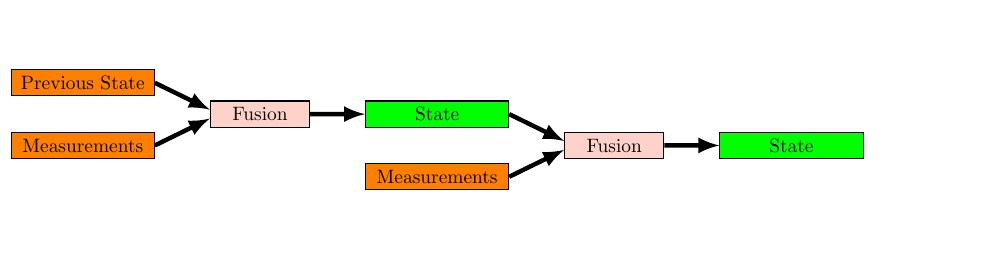
\begin{tikzpicture}[scale=\scalefilter, every node/.style={transform shape}]
\path [draw=none, use as bounding box] (0,0) rectangle (17,4);

\node (A) at (1,3) [input, fill=\initialstatecolor] {\initialstatetext};
\node (dummy1) [dummy, below=2mm of A] {};
\node (C) [input,below=2mm of dummy1] {Measurements};
\node (D) [method,right=of dummy1] {Fusion};
\node (E) [input, right=of D, fill=\nodestatecolor] {State};

\node<2-> (dummy2) [dummy, below=2mm of E] {};
\node<2-> (F) [input, below=2mm of dummy2] {Measurements};


\node<3-> (G) [method, right=of dummy2] {Fusion};
\node<3-> (H) [input, right=of G, fill=green] {State};

\draw[arr] (A.east) -- (D.175);
\draw[arr] (C.east) -- (D.185);
\draw[arr] (D.east) -- (E.west);
\draw<3->[arr] (E.east) -- (G.175);
\draw<3->[arr] (F.east) -- (G.185);
\draw<3->[arr] (G.east) -- (H.west);

\end{tikzpicture}
}

\onslide<4->
How to recover the \textbf{initial state}?

\onslide<5->
We need a \textbf{deterministic solution}

\vspace{0.5cm}
{\centering
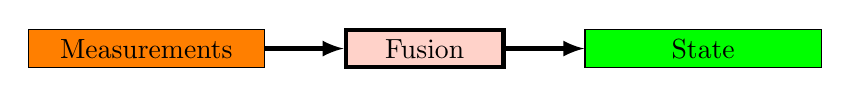
\begin{tikzpicture}
\tikzstyle{input}=[draw,fill=myyellow,minimum width=3cm,thin]
\tikzstyle{method}=[draw,fill=mypink,minimum width=2cm]
\tikzstyle{every path}=[-latex,ultra thick]
\node (C) [input] {Measurements};
\node (D) [method,right=of C] {Fusion};
\node (E) [input, right=of D, fill=green] {State};



\draw (C.east) -- (D.west);
\draw (D.east) -- (E.west);
\end{tikzpicture}
}

\end{frame}

\begin{frame}{The Closed-Form Solution}

  \begin{flushright}
    \small
    Transactions on Robotics (T-RO) 2012\\
    International Journal of Computer Vision (IJCV) 2014
  \end{flushright}

  \onslide<2->

  %% \vspace{-1em}

  \textbf{Theory}:

  \only<5->{\renewcommand*\themethod{Non-linear optimization}}
  {\centering
    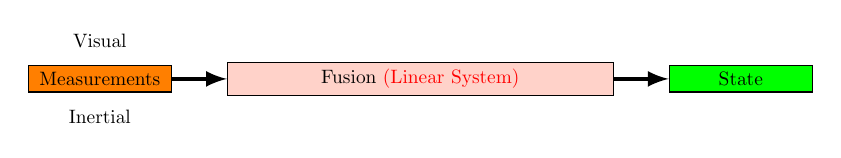
\begin{tikzpicture}[scale=\scalefilter, every node/.style={transform shape}]
      \node (A) [input, fill=myyellow] {Measurements};
      \node (B) [above=2mm of A] {Visual};
      \node (C) [below=2mm of A] {Inertial};
      \node (D) [method,right=of A, minimum width=7cm] {Fusion \textcolor{red}{(\themethod)}};
      \node (E) [input, right=of D, fill=\nodestatecolor] {State};
      \draw[arr] (A.east) -- (D.west);
      \draw[arr] (D.east) -- (E.west);
    \end{tikzpicture}
  }


  \onslide<3->{
    \hrulefill

    \textbf{Practice}:
  }

  \begin{overlayarea}{\textwidth}{0.6\textheight}

    \includegraphics<3>[width=0.4\textwidth]{images/droneCrash.png}

    \begin{columns}<4>
      \begin{column}{.5\textwidth}
        \centering
        Acclerometer bias?

        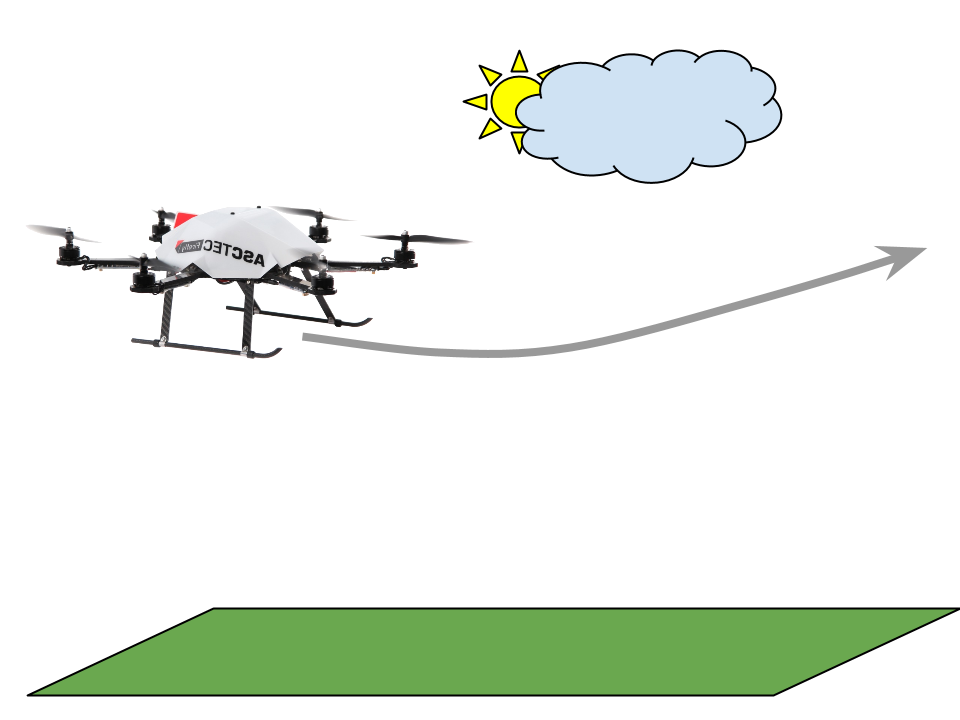
\includegraphics[width=0.8\textwidth]{images/droneFly.png}
      \end{column}
      \vrule{}
      \begin{column}{.5\textwidth}
        \centering
        Gyroscope bias?

        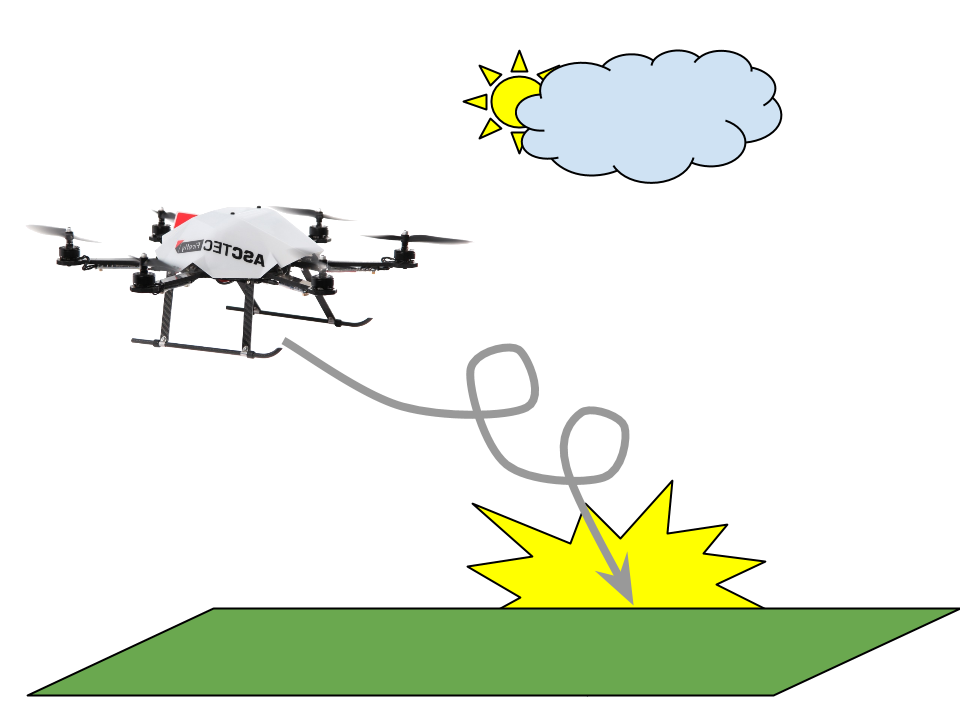
\includegraphics[width=0.8\textwidth]{images/droneCrash.png}
      \end{column}
    \end{columns}

    \vspace{-3.65cm}

    \onslide<5> \textbf{Optimization} to recover the gyroscope bias

    \includegraphics<5>[width=0.4\textwidth]{images/droneFly.png}

  \end{overlayarea}

\end{frame}

\begin{frame}[plain,c]
  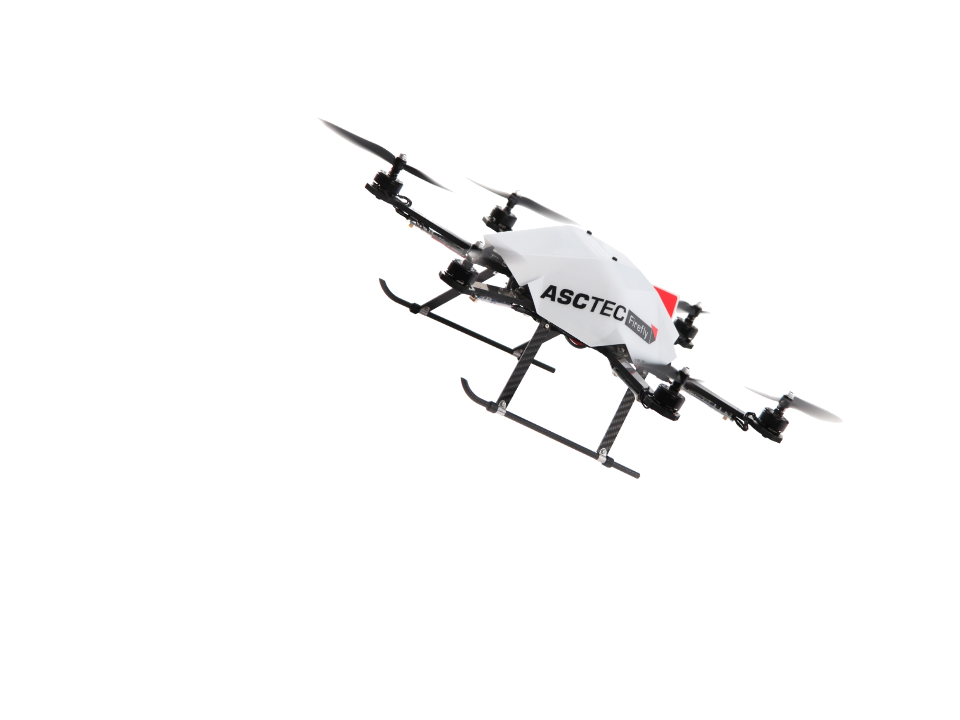
\includegraphics[width=0.6\textwidth]{images/drone.png}

  \begin{center}
    Thank you for your attention,\\
    come visit our poster
  \end{center}
\end{frame}

\end{document}
